\section{Background}\label{sec:ccg}
Language comprehension could be briefly stated as the process of transforming words into meaning. Language production is the opposite process. Language production thus consists of several tasks, including transforming some semantic representation into words, and then combining those words into ideas. For now, we primarily focus on the second task, which we accomplish with a grammar formalism, \textit{Combinatory Categorial Grammar} (CCG) \citep{ccg}.

CCG is a grammar in the family of mildly-context sensitive grammars, along with Tree-Adjoining Grammar \citep{tag}. Mildly-context sensitive grammars have been shown to be capable of representing human speech, and computationally plausible in real-time \citep{convergence}. Also importantly, CCG stores only a single type value at any given point for combined words, as opposed to TAG which stores the entire tree. The types in CCG can be arbitrarily complex, but its rules are quite simple. See Figure~\ref{eqn:ccg} for a demonstration of the rules. See Figure~\ref{fig:ccg} for an example of a derivation.

\begin{figure}
\[X/Y > Y = X\]
\[Y < X\setminus Y = X\]
\[X/Y >> Y/Z = X/Z\]
\[Y\setminus Z << X\setminus Y = X\setminus Z\]
\caption{Forward Application, Backward Application, Forward Composition, and Backward Composition respectively. Note that types $A,B$ could be any of combinatorially derived types of CCG}
\label{eqn:ccg}
\end{figure}

\begin{figure}[ht]
\begin{center}
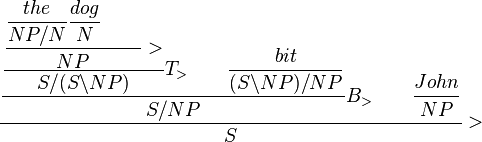
\includegraphics[width=0.95\columnwidth]{figures/ccg}
\end{center}
\caption{An example of a derivation of CCG. Note that the $T>$ is for type-raising, which is handled my declarative memory rather than production rules in my model. \textbf{Redo with my own application combinators}}  
\label{fig:ccg}
\end{figure}

\section{Model}
The presented model is implemented in jACT-R \citep{jactr}, a full Java implementation of the ACT-R theory \citep{actr}. Unlike other potential variants \citep{actup}, jACT-R has the same full set of constraints as ACT-R.  

The presented model's chunks and productions presently largely have a one to one correspondence with CCG. The primary production rules besides memory retrievals are rules directly from CCG; the primary computational units are the types in CCG.  

In theory, a model of language production should not make any more assumptions beyond ACT-R, in practice, the model relies on several simplifications. In the future, many of these could become parameters to a model to compare how well the model fits. The model's basic goal is to greedily combine lexical-syntactic chunks together to form a sentence. Right now, the process for that combination consists of the syntactic rules of CCG, and the model has no inherent preference for what to combine with what, besides as described later in experiments.

\subsection{Rules and Chunks}
The model itself, due to its ability to generalize to any sentence, is programatically generated. The model has \textit{classes} of rules and classes of chunks. A general layout of the production rules can be found in Figure~\ref{fig:prod}. The organizational scheme of the chunks can be found in Figure~\ref{fig:dm}.

\subsubsection{Production Rules}\label{sec:rules}
There are several classes of production rules. A class of production rules can be thought of as a type of operation, with each specific production rule being that operation on that chunk. For instance, it takes two separate production rules to combine two elements that are at different points in the sentence. Secondly, it takes a different production rule to determine which of the types the Lexsyn should use to combine. For instance, family can be either an adjective or a noun, and it could fill a slot earlier in the sentence ("My family and I went to eat dinner") or later ("I went with my family members to eat dinner"). The main classes of production rules are as follows:
\begin{itemize}
\item Move word $A$ into the model: The word moves from DM into the goal buffer. This class contains position information, so there are $N$ of them, where $N$ is the number of words in the sentence.
\item Retrieve lexsyn $A_{lex}$ for the word $A$: The type info moves from DM into the goal buffer. This class contains position information, so there are $N$ of them, where $N$ is the number of words in the sentence.
\item Apply Syntactic Rule to $A_{lex}$ and $B_{lex}$: CCG defines four basic and a few more complicated syntactic rules, which are described in Section~\ref{sec:ccg}. This class contains position and type information both two arguments, so there are $N * K * (N-1) * J$, where $N$ is the number of words in the sentence, $K$ is the number of types $A_{lex}$ has, and $J$ is the number of types $B_{lex}$ has
\item Resolve Syntactic Rule on $A_{lex}$: In this step, the new type that results from the previous operation is retrieved and stored in $A_{lex}$, and $B_{lex}$ is removed from the goal buffer.
\item Terminate and begin new sentence: If only a single lexsyn remains because all of them have been successfully combined, or no more rules are applicable, then the sentence is finished and the model will start its next goal. 
\end{itemize}

\subsubsection{Declarative Memory}\label{sec:dm}
Declarative Memory is composed of a few simple chunk types, described below.
\begin{itemize}
\item Word : A word simply has a name, which corresponds to its lexical information (e.g. family).
\item Type : A type is an arbitrarily complicated CCG type. The types that exist in DM are the types that are used in the Switchboard CCG derivations.
\item Lexsyn : A Lexsyn associates a Word with some number of Types. The chosen types are the types that the word has in the Switchboard corpus, including from type-raising.\footnote{Type-raising is a CCG operation where a type changes to a symbolically different but effectively equivalent type. This allows derivations in different orders.}
\item Sentence : A sentence is the work area to create the final utterance. Thus, it starts with words, which eventually become several Lexsyns, which eventually combine into a single Lexsyn, representing the finished sentence.
\end{itemize}

\begin{figure}[ht]
\begin{center}
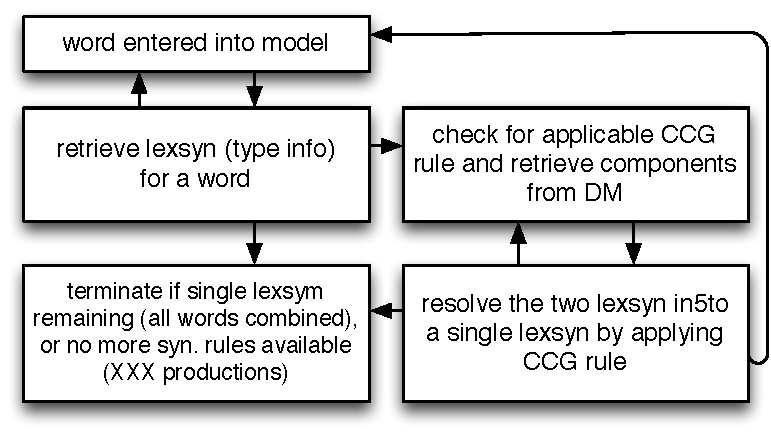
\includegraphics[width=0.95\columnwidth]{figures/model-FSA}
\end{center}
\caption{General process flow of the production rules of the model. See Section~\ref{sec:rules} for a more detailed description.}  
\label{fig:prod}
\end{figure}

\begin{figure}[ht]
\begin{center}
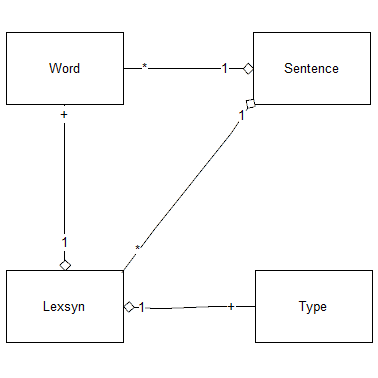
\includegraphics[width=0.95\columnwidth]{figures/prodtypes}
\end{center}
\caption{General data model of the declarative memory. See Section~\ref{sec:dm} for a more detailed description.}  
\label{fig:dm}
\end{figure}

\subsection{Input}
Normally, to simulate language production, we would prefer the model start with a semantic representation. Unfortunately, starting with a true semantic representation requires both an evaluation of that representation and an implementation of lexical selection. Thus, we used a simple proxy for the semantic representation as an unordered set of words that could create at least one valid sentence. The words are taken from sentences in the Switchboard corpus.

\subsection{Output}
The model attempts to produce a sentence. However, it does not always successfully finish a sentence, sometimes producing a fragment or several disconnected fragments.

\subsection{Evaluation}
Naturally, while the model produces utterances, those utterances don't always make sense. Quantifying exactly what it is to make sense is obviously difficult, so we went with a simpler metric: what is probable. We scored each sentence using a weighted bigram average using the SRILM toolkit trained on the spoken BNC corpus \citep{srilm} inspired by \citet{chart}. While we could have compared the utterance to the original sentence, since we are mostly bypassing the semantic representation component, we are more concerned with the model producing any good utterances, rather than the ones with the intended meaning.
